%%%%%%%%%%%%%%%%%%%%%%%%%%%%%%%%%%%%%%%%%
% Stylish Article
% LaTeX Template
% Version 2.2 (2020-10-22)
%
% This template has been downloaded from:
% http://www.LaTeXTemplates.com
%
% Original author:
% Mathias Legrand (legrand.mathias@gmail.com) 
% With extensive modifications by:
% Vel (vel@latextemplates.com)
%
% License:
% CC BY-NC-SA 3.0 (http://creativecommons.org/licenses/by-nc-sa/3.0/)
%
%%%%%%%%%%%%%%%%%%%%%%%%%%%%%%%%%%%%%%%%%

%----------------------------------------------------------------------------------------
%	PACKAGES AND OTHER DOCUMENT CONFIGURATIONS
%----------------------------------------------------------------------------------------

\documentclass[fleqn,10pt]{SelfArx} % Document font size and equations flushed left

\usepackage[english]{babel} % Specify a different language here - english by default

\usepackage{lipsum} % Required to insert dummy text. To be removed otherwise

%----------------------------------------------------------------------------------------
%	COLUMNS
%----------------------------------------------------------------------------------------

\setlength{\columnsep}{0.55cm} % Distance between the two columns of text
\setlength{\fboxrule}{0.75pt} % Width of the border around the abstract

%----------------------------------------------------------------------------------------
%	COLORS
%----------------------------------------------------------------------------------------

\definecolor{color1}{RGB}{0,0,90} % Color of the article title and sections
\definecolor{color2}{RGB}{0,20,20} % Color of the boxes behind the abstract and headings

%----------------------------------------------------------------------------------------
%	HYPERLINKS
%----------------------------------------------------------------------------------------

\usepackage{hyperref} % Required for hyperlinks

\hypersetup{
	hidelinks,
	colorlinks,
	breaklinks=true,
	urlcolor=color2,
	citecolor=color1,
	linkcolor=color1,
	bookmarksopen=false,
	pdftitle={Title},
	pdfauthor={Author},
}

%----------------------------------------------------------------------------------------
%	ARTICLE INFORMATION
%----------------------------------------------------------------------------------------

\JournalInfo{Assignment 2 - Machine Learning for Natural Language Processing} % Journal information
\Archive{Fall Semester 22} % Additional notes (e.g. copyright, DOI, review/research article)

\PaperTitle{Word Embedding Based on Hotel Reviews and Sci-Fi Stories - The Continuous Bag of Words Approach} % Article title



\Keywords{CBOW --- Word2Vec --- Natural Language Processing} % Keywords - if you don't want any simply remove all the text between the curly brackets
\newcommand{\keywordname}{Keywords} % Defines the keywords heading name

%----------------------------------------------------------------------------------------
%	ABSTRACT
%----------------------------------------------------------------------------------------

\Abstract{One of the most important inventions in the world of Natural Language Processing (NLP) is probably the representation of words as vectors. These so-called Word Embeddings (WE) manage to encapsulate the meaning of words and the proximity to other words in the form of numbers. To create these WEs, neural network and dimensionality reduction techniques are employed. The training data used by such models can represent any type of text. For example, well-known models in the past made use of data from Wikipedia. In the following, we outline our work in which we created our own WE using the Continuous Bag of Words (CBOW) approach. For model Training we use Trip-Advisor Reviews and a SciFi story.}

%----------------------------------------------------------------------------------------

\begin{document}

\maketitle % Output the title and abstract box

\tableofcontents % Output the contents section

\thispagestyle{empty} % Removes page numbering from the first page

%----------------------------------------------------------------------------------------
%	ARTICLE CONTENTS
%----------------------------------------------------------------------------------------

\section{Introduction} % The \section*{} command stops section numbering
This is our report for the second assignment of the Machine Learning for Natural Language Processing 1 course. The task was to train CBOW Embeddings on both data from Hotel Reviews and Sci-Fi Stories. The goal of this exercise is to:
\begin{itemize}[noitemsep] % [noitemsep] removes whitespace between the items for a compact look
	\item understand the basic building blocks for training models in PyTorch.
	\item understand what word embeddings are and how you train them.
	\item think about how one can evaluate word embeddings
\end{itemize}

%------------------------------------------------

\section{Data \& Task Description}

\subsection{Data}
We will work with the complete “Trip Advisor hotel reviews” and “Sci-fi stories” for this exercise. One can Download the datasets from the material folder in the exercise section of OLAT. The folder contains the files “tripadvisor\_hotel\_reviews.csv” and “scifi.txt”. The files are also hosted under the following links:

\begin{itemize}[noitemsep] % [noitemsep] removes whitespace between the items for a compact look
	\item tripadvisor\_hotel\_reviews.csv:
	
	https://drive.google.com/file/d/1ihP1HZ8YHVGGIEp1RH \linebreak xXdt3PPIi12xvL/view?usp=sharing
	\item scifi.txt:
	
	https://drive.google.com/file/d/10ehW4jZND3QA29v9aNbo \linebreak YUett5-swuNe/view?usp=sharing
\end{itemize}
The above URL can be used to load the data directly in your Colab notebook - as you already did in Exercise 1.

\subsection{Task 1 - Train your CBOW embeddings for both datasets}
Go to this Colaboratory Python Notebook (homepage from where we took it), create a copy of it and complete the missing code in the exercise section - which means implementing a CBOW model in PyTorch. Then, change the code so that it takes the Trip advisor hotel reviews text as input and produces word embeddings for the hotel reviews.

We strongly recommend (but do not require) an OOP-oriented approach e.g. as presented in Chapter 3 from Rao and
McMahan. If you follow Rao and McMahan, that means building the classes for the vectorizer, data loader, etc. Make sure
that the code is understandable by either using comments for classes and methods or by explaining the code in text cells of the notebook.

It is up to you to decide on the specific preprocessing steps (removing punctuation, lower-casing, numbers etc.).
Describe your decisions (preprocessing, class structure) in the lab report.

You will train two models:
\begin{enumerate}[noitemsep]
    \item CBOW2 with a context width of 2 (in both directions) for the Hotel Reviews dataset
    \item and CBOW2 with a context width of 2 (in both directions) for the Sci-Fi story dataset.
\end{enumerate}


In order to obtain useful embeddings without training too long we recommend an embedding size of 50 and 12-15 epochs
on the hotel reviews dataset. On the Sci-fi dataset 2 epochs are enough. And if you want, you can always try larger embedding sizes with more epochs.

\paragraph{optimal} Train CBOW5 with a context width of 5 (in both directions). Are predictions made by the model sensitive towards the context size? This paper \href{https://aclanthology.org/I17-2006/}{(here)} provides an insight on how to choose a minimum embedding size while still obtaining useful representations.

Note: Training may take multiple hours. If you have been inactive in the Colab environment for a certain period of time Colab may regard your user session as idle and disconnect - which disrupts the training. To prevent that from happening tricks like \href{https://gist.github.com/RodolfoFerro/a12c664330c6eae601e5a828adfb8306}{this} help.

\subsection{Task 2 - Test your embeddings}
Word embeddings are not easy to evaluate automatically without suitable test sets. For this exercise, we inspect them manually to get a feel for whether they capture what we think they should capture. Computing the nearest neighbours (see below) for a word allows us to get an intuition on the semantic vector space. Do the following for CBOW2 and, optionally, for CBOW5:

\begin{enumerate}[noitemsep]
    \item For the hotel reviews dataset choose 3 nouns, 3 verbs, and 3 adjectives. Make sure that some of the nouns/verbs
    /adjectives occur frequently in the corpus and that others are rare. For each of the 9 chosen words, retrieve the 5 closest words according to your trained CBOW2 model. List them in your report and comment on the performance of your model: do the neighbours the model provides make sense? Discuss.
    \item Repeat what you did in 2. for the Sci-fi dataset.
    \item How does the quality of the hotel review-based embeddings compare with the Sci-fi-based embeddings? Elaborate.
    \item Choose 2 words and retrieve their 5 closest neighbours according to hotel review-based embeddings and the Sci-fi-based embeddings. Do they have different neighbours? If yes, can you reason why?
    \item (optional) What are the differences between CBOW2 and CBOW5 (if trained)? Can you "describe" them?
\end{enumerate}

\section{Data Preprocessing}
\subsection{Trip Advisor Dataset}
The Trip advisor dataset includes hotel reviews, which were stated on Trip Advisor, along with labels that indicate how much the reviewer enjoyed the trip. The scale of the label allows 5 values between 1 and 5, 1 is the worst rating, indicating the reviewer was not satisfied at all, and 5 is the best rating, meaning the reviewer was very satisfied. 
The data is encapsulated in a loader class. This class is  used for loading the data from the provided link (see section Data \& Task Description) and for preprocessing. The loader class is then composed into a dataset class, which inherited from pytorch  \href{https://pytorch.org/tutorials/beginner/basics/data_tutorial.html}{Dataset}. The dataset class was then composed into a dataloader class, which allowed for batched training. 

The data was preprocessed according to the following pipeline:
\begin{enumerate}[noitemsep]
    \item Even though casing can be very important in some embeddings, we decided not to use the linguistic usage of a word for context, but to focus more on the meaning. Simply put, not lowercasing results in the position of a word in the sentence being taken into account in the embedding. Lowercasing prevents this and results in only the meaning of the word being embedded. This was done so that the embeddings do not take into account the structure of the sentence.
    \item Second, white spaces was striped from the data. 
    \item Third, numbers were deleted from the training data because they are mostly substitutable. The number 2022 can be used in many different contexts, each with a different meaning. E.g. what is the result of 4044/2 ? 2022; In which year are we right now? 2022. Word embeddings have great difficulty with such ambiguities. There are two ways to deal with the problem: Either one simply deletes the numbers, or one can replace them with a tag (e.g. [NUMBER]). We have chosen the first option.
    \item All punctuation marks have been removed. This is closely related to point 4. Essentially, we want to focus the embeddings on the meaning of a word and not on its position in the sentence.
    \item Individual subsets were segmented. This is because it is an open secret that embeddings across sentences work very poorly. Reviews often come in partial sentences: "Very great hotel right by the sea, the food was very good, we also liked the staff a lot." Each of these partial sentences embodies its own statement. If we were to train CBOW across these commas (sub-sentences), we would embed a wild tangle of meaning into the vector representations.
    \item Next, Unicode Normalization (UN) was applied. ”Programs should always compare canonical-equivalent Unicode strings as equal” (https://www.unicode.org/faq/
    normalization.html). This ensures better comparability of similar words/phrases utilizing different Unicode encodings. We used the ”unicodedata” library (https://docs.python.org/3/library/unicodedata.html) to perform UN.
    \item Lastly, spelling correction was applied. Especially in user reviews, it is very likely that spelling errors occur. For this purpose, we made use of the Caribe library. Which, though computationally very expensive, provides very high quality sentence correction (https://www.thecaribe.org/). In oppose to other spelling correction engines (such as pyspellchecker), Caribe operates at sentence level and not at single word level.
\end{enumerate}

\subsection{Sci-Fi Stories}
The SciFi data set came in .txt format. As the name suggests, the file included a full science fiction story. The data was read into python directly through the provided link (see section Data & Task Description). Similar to the Trip-Advisor dataset, the SciFi dataset was brought into tabular format. Each row encapsulates a single sentence of the science fiction story. This ensures that the training data strictly consists of contexts belonging to the same sentence. In the following, the preprocessing pipeline is outlined:

\begin{enumerate}[noitemsep]
    \item The first and the last 15 rows of the dataset are deleted. These rows contain metadata about the document, which, due to lack of meaningfulness, isn’t of use when training WEs.
    \item Second, the data is lowercased and whitespaces are striped. Reasons for both are described in the preprocessing section of the Trip-Advisor dataset.
    \item Third, backslashes (\textbackslash) and hashtags (\#) are removed. Both are used for correct machine interpretation. For WEs, these characters are of no use. One might argue that some special characters, such as ‘ (we’re, don’t, he’s) are of great importance in the English language. While we are aware of this, we argue that with equivalent preprocessing of the training data and the later words when their embedding will be retrieved, this is not problematic. For example, a user might want to retrieve the embedding for the word “don’t”. His word would automatically be preprocessed with the same pipeline as the training data and would only then be shown to the model.
    \item All signs and digits are deleted from the dataset. Reasons for this are discussed in the preprocessing section for the Trip-Advisor dataset. Essentially, we believe that most numbers (such as years) are ambiguous, which, as discussed in the lecture, is a weakness of WEs.
    \item From the previous preprocessing steps, there are now some corrupt rows in the data. For example, the row: “@#!!”, which represents a curse word, is now empty. We define the criterion for such corrupted lines as those, which have less than three words in them. This is, of course, not a perfect criterion as some non-corrupt lines are also expected to have no more than two words. But considering our training data has around 1.2 million rows, dropping some non-corrupt lines might not be so problematic. 
    \item Lastly, UN is performed. Reasons are described in the preprocessing section of the Trip-Advisor dataset.
\end{enumerate}

\section{Class Structure}
As recommended in the exercise sheet, we applied an object oriented approach. For each data set, we used a custom loader class, which automatically downloads and reads the data, and then applies the preprocessing steps. This loader class was then composed into dataset class, which inherits from Pytorch's Dataset module. The inherited class was then converted to a DataLoader, which makes it easy to train the model in batches. The dataset classes both used tensor representations to store the data. This comes with the advantage of \href{https://de.wikipedia.org/wiki/CUDA}{CUDA} acceleration.

Further we have defined a class with all utility methods. Here we specifically mention the method make\_word\_dict\_and \_data(). It is apparent from the method that we do not extract training data beyond sentences (for reasons see preprocessing). The review "The hotel was very nice, The restaurant had a very high standard." did, for example, not result in the training set:  ([nice, the, had, a], restaurant), as it was treated as two sentences.

For the CBOW model, we applied the object-oriented Pytorch approach as described in \href{https://b-ok.global/book/3711505/debacd}{Rao and McMahan}. The CBOW model inherits from the nn.Module, which provides many important functionalities for our purpose.

The training loop is packed into a class called ModelTrainer. This class makes it easy to train our models and avoid code duplications. 

\section{Theory - Continuous Bag of Words}

\paragraph{Word Embeddings: Encoding Lexical Semantics}

Word embeddings are dense vectors of real numbers, one per word in your vocabulary. In NLP, it is almost always the case that your features are words! But how should you represent a word in a computer? You could store its ascii character representation, but that only tells you what the word \textit{is}, it doesn't say much about what it \textit{means} (you might be able to derive its part of speech from its affixes, or properties from
its capitalization, but not much). Even more, in what sense could you combine these representations? We often want dense outputs from our neural networks, where the inputs are $|V|$ dimensional, where $V$ is our vocabulary, but often the outputs are only a few dimensional (if we are only predicting a handful of labels, for instance). How do we get from a massive dimensional space to a smaller dimensional space?

How about instead of ascii representations, we use a one-hot encoding?
That is, we represent the word $w$ by

\begin{align} \overbrace{\left[ 0, 0, 0, 0, \dots, \dots, \dots, 1, \dots, \dots, \dots, 0, 0, 0, 0 \right]}^\text{$|V|$ elements} \end{align}

where the 1 is in a location unique to $w$. Any other word will have a 1 in some other location, and a 0 everywhere else.

There is an enormous drawback to this representation, besides just how huge it is. It basically treats all words as independent entities with
no relation to each other. What we really want is some notion of \textit{similarity} between words. Why? Let's see an example.

Suppose we are building a language model. Suppose we have seen the sentences:

\begin{itemize}[noitemsep]
    \item The mathematician ran to the store
    \item The physicist ran to the store.
    \item The mathematician solved the open problem.
\end{itemize}

in our training data. Now suppose we get a new sentence never before seen in our training data:

\begin{itemize}[noitemsep]
    \item The physicist solved the open problem.
\end{itemize}

Our language model might do OK on this sentence, but wouldn't it be much better if we could use the following two facts:

\begin{itemize}[noitemsep]
    \item We have seen  mathematician and physicist in the same role in a sentence. Somehow they have a semantic relation.
    \item We have seen mathematician in the same role  in this new unseen sentence as we are now seeing physicist.
\end{itemize}

and then infer that physicist is actually a good fit in the new unseen sentence? This is what we mean by a notion of similarity: we mean
\textit{semantic similarity}, not simply having similar orthographic representations. It is a technique to combat the sparsity of linguistic
data, by connecting the dots between what we have seen and what we haven't. This example of course relies on a fundamental linguistic assumption: that words appearing in similar contexts are related to each other semantically. This is called the \href{https://en.wikipedia.org/wiki/Distributional_semantics} {distributional hypothesis}.


\paragraph{Getting Dense Word Embeddings} How can we solve this problem? That is, how could we actually encode semantic similarity in words? Maybe we think up some semantic attributes. For example, we see that both mathematicians and physicists can run, so maybe we give these words a high score for the "is able to run" semantic attribute. Think of some other attributes, and imagine what you might score some common words on those attributes.

If each attribute is a dimension, then we might give each word a vector, like this:

\begin{align}q_\text{mathematician} = \left[ \overbrace{2.3}^\text{can run},\overbrace{9.4}^\text{likes coffee}, \overbrace{-5.5}^\text{majored in Physics}, \dots \right]\end{align}

\begin{align}q_\text{physicist} = \left[ \overbrace{2.5}^\text{can run}, \overbrace{9.1}^\text{likes coffee}, \overbrace{6.4}^\text{majored in Physics}, \dots \right]\end{align}

Then we can get a measure of similarity between these words by doing:

\begin{multline}\text{Similarity}(\text{physicist}, \text{mathematician}) = \\
q_\text{physicist} \cdot q_\text{mathematician}\end{multline}

Although it is more common to normalize by the lengths:

\begin{multline}\text{Similarity}(\text{physicist}, \text{mathematician}) = \\ 
\frac{q_\text{physicist} \cdot q_\text{mathematician}}{\| q_\text{\physicist} \| \| q_\text{mathematician} \|} = \cos (\phi)\end{multline}

Where $\phi$ is the angle between the two vectors. That way, extremely similar words (words whose embeddings point in the same direction) will have similarity 1. Extremely dissimilar words should have similarity -1.

You can think of the sparse one-hot vectors from the beginning of this section as a special case of these new vectors we have defined, where each word basically has similarity 0, and we gave each word some unique semantic attribute. These new vectors are \textit{dense}, which is to say their entries are (typically) non-zero.

But these new vectors are a big pain: you could think of thousands of different semantic attributes that might be relevant to determining
similarity, and how on earth would you set the values of the different attributes? Central to the idea of deep learning is that the neural
network learns representations of the features, rather than requiring the programmer to design them herself. So why not just let the word
embeddings be parameters in our model, and then be updated during training? This is exactly what we will do. We will have some \textit{latent semantic attributes} that the network can, in principle, learn. Note that the word embeddings will probably not be interpretable. That is,
although with our hand-crafted vectors above we can see that mathematicians and physicists are similar in that they both like coffee,
if we allow a neural network to learn the embeddings and see that both mathematicians and physicists have a large value in the second
dimension, it is not clear what that means. They are similar in some latent semantic dimension, but this probably has no interpretation to
us.

In summary, \textit{word embeddings} are a representation of the \textit{semantics} of a word, efficiently encoding semantic information that might be relevant to the task at hand. You can embed other things too: part of speech tags, parse trees, anything! The idea of feature embeddings is central to the field.

\paragraph{Continuous Bag of Words} The Continuous Bag-of-Words model (CBOW) is frequently used in NLP deep learning. It is a model that tries to predict words given the context of a few words before and a few words after the target word. This is distinct from language modeling, since CBOW is not sequential and does not have to be probabilistic. Typcially, CBOW is used to quickly train word embeddings, and these embeddings are used to initialize the embeddings of some more complicated model. Usually, this is referred to as \textit{pretraining embeddings}. It almost always helps performance a couple of percent.

The CBOW model is as follows: Given a target word $w_i$ and an $N$ context window on each side, $w_{i-1}, \dots, w_{i-N}$ and $w_{i+1}, \dots, w_{i+N}$, referring to all context words collectively as $C$, CBOW tries to minimize

\begin{align}-\log p(w_i | C) = -\log \text{Softmax}(A(\sum_{w \in C} q_w) + b)\end{align}

where $q_w$ is the embedding for word $w$.

\section{Model Training}

\subsection{Trip-Advisor Data Model}
The Trip-Advisor data CBOW was trained over 12 epochs. The data was loaded in batches of 4 observations using PyTorch Dataloader. The total loss converged nicely as evident from Figure \ref{fig:ta-loss}. The computation was executed on an NVIDIA Tesla K80 using CUDA. The training time was 3h 24min, during which the GPU had an average usage of around 82\% (see Figure \ref{figure:ta-gpuusage}).
\begin{figure}[ht]\centering
	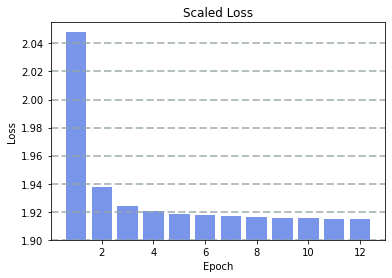
\includegraphics[width=\linewidth]{Figures/Model1 Loss.png}
	\caption{Trip-Advisor CBOW: Scaled loss per epoch. Total loss was divided by the number of observations}
	\label{fig:ta-loss}
\end{figure}
\begin{figure}[ht]\centering
	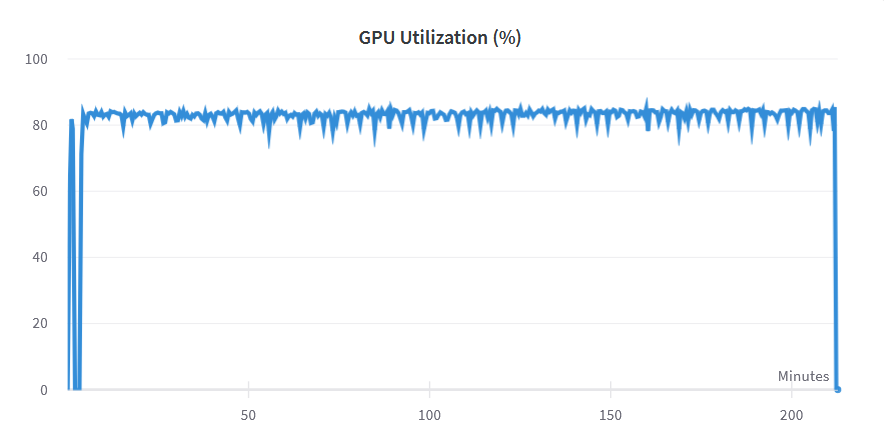
\includegraphics[width=\linewidth]{Figures/GPU Utilization.png}
	\caption{Trip-Advisor CBOW: GPU usage over time.}
	\label{figure:ta-gpuusage}
\end{figure}

\subsection{SciFi Data Model}
The SciFi data CBOW was trained over 12 epochs. This is mainly due to the huge size of the training data. To further reduce the training time, we down-sampled the dataset from 1.2 million rows to 100'000 rows. The data was loaded in batches of 4 observations using PyTorch Dataloader. The total loss converged nicely as evident from Figure \ref{fig:sf-loss}. The computation was also executed on an NVIDIA Tesla K80 using CUDA. The training time was 2h 36min, during which the GPU had an average usage of around 93\%.
\begin{figure}[ht]\centering
	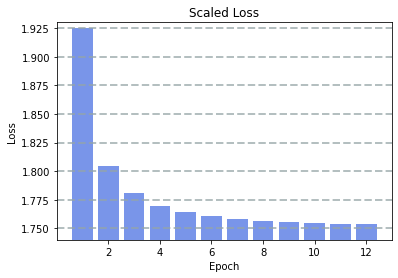
\includegraphics[width=\linewidth]{Figures/Model2 Loss.png}
	\caption{SciFi CBOW: Scaled loss per epoch. Total loss was divided by the number of observations}
	\label{fig:sf-loss}
\end{figure}
\section{Results}
As word embeddings are not easy to evaluate automatically without suitable test sets, we inspected them manually. Therefor the nearest neighbours were computed using a code snippet provided by the teaching staff. 3 nouns, 3 verbs and 3 adjectives were chosen for both datasets in order to evaluate their nearest neighbours. The words were selected according to their frequency to ensure that both common and rare words were chosen.  Figure \ref{fig:hotelwords} and \ref{fig:scifiwords} show the word selection, including their frequency.
\begin{figure}[ht]\centering
	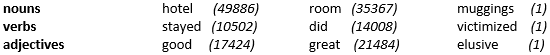
\includegraphics[width=\linewidth]{Figures/hotel_words.png}
	\caption{Word choices for the hotel review data set, with their frequency in parentheses.}
	\label{fig:hotelwords}
\end{figure}

\begin{figure}[ht]\centering
	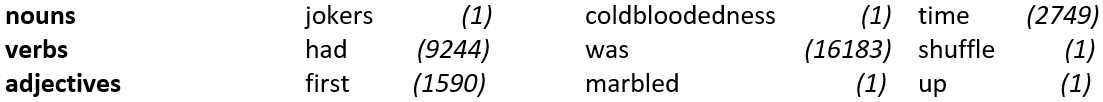
\includegraphics[width=\linewidth]{Figures/scifi_words.png}
	\caption{Word choices for the Sci-fi story data set, with their frequency in parentheses.}
	\label{fig:scifiwords}
\end{figure}

\noindent Figure \ref{fig:hotel_results} and \ref{fig:scifi_results} show the results obtained based on the two word selections. Figure \ref{fig:scifi_results} refers to the model trained with the sci-fi data and Figure \ref{fig:hotel_results} shows the closest words according to the model trained on the hotel reviews. The distance was rounded to 2 decimal places.

\begin{figure}[ht]\centering
	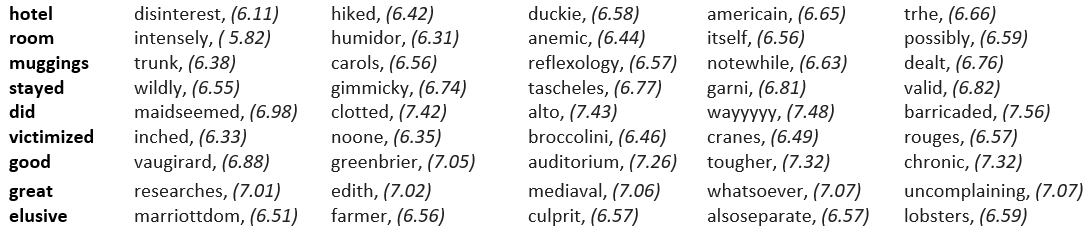
\includegraphics[width=\linewidth]{Figures/hotel_results.png}
	\caption{Five closest words according based on the words shown in Figure \ref{fig:hotelwords} and their distance.}
	\label{fig:hotel_results}
\end{figure}

\begin{figure}[ht]\centering
	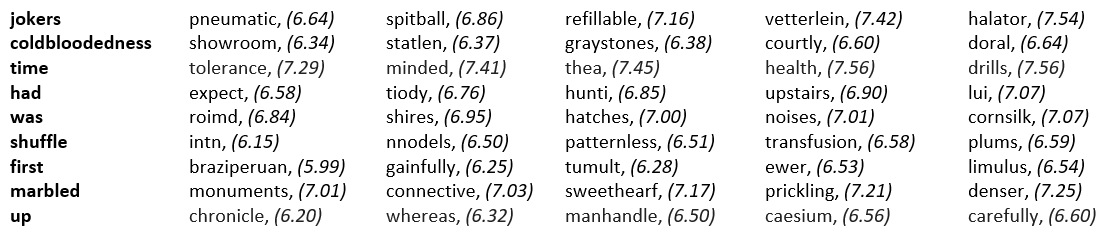
\includegraphics[width=\linewidth]{Figures/scifi_results.png}
	\caption{Five closest words according based on the words shown in Figure \ref{fig:scifiwords} and their distance.}
	\label{fig:scifi_results}
\end{figure}
\noindent Further the two models were directly compared, using the words "the" and "good". Their closest five closest neighbours were retrieved according to both models, to allow a comparison between them. This is illustrated in Figure \ref{fig:comparison}. As in the previous tables, the distance was rounded to 2 decimal places. The results are discussed in the following chapter.
\begin{figure}[ht]\centering
	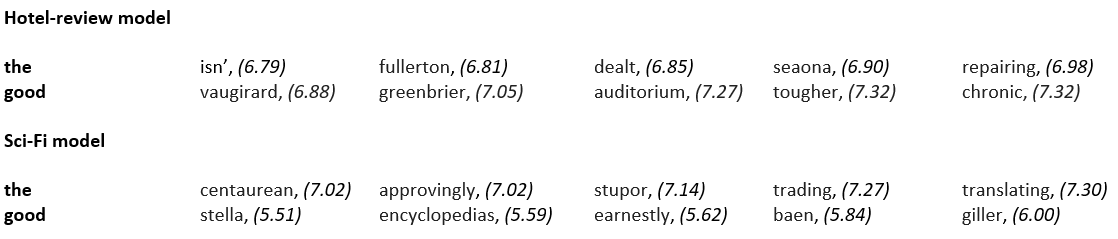
\includegraphics[width=\linewidth]{Figures/comparison.png}
	\caption{Comparison of the two models using the words "good" and "the".}
	\label{fig:comparison}
\end{figure}

\section{Discussion}
Having a look at figures \ref{fig:scifi_results} we see that some neighbours (e.g. chronicle, ewer or transfusion) are terms that are related to the field of sci-fi. However there are also a lot of non-field-specific neighbours such as expect, showroom or spitball. In fact the majority of words don't seem to be typical words for sci-fi literature or words that one would intuitively link to sci-fi. The same can be said of \ref{fig:hotel_results}. Here the results seem to be even more vague. It is hard to see how "anemic" or "reflexology" would relate to hotel reviews.
\newline
\newline
The direct comparison using the words "the" and "good" provided interesting results. As expected, the two models resulted in different outputs. This makes sense, because the first model was trained on hotel-review data, while the second model was trained on sci-fi texts. These two topics differ majorly and only have few interfaces. Therefor one can expect at least some minor (if not major) differences in the closest neighbours suggested by the models.
\newline
\newline
Inspecting the results of the model trained on the Sci-fi data in Figure 8 one can see that two of the closest neighbours are especially interesting: 1. Centaurean and 2. Bean. Bean books is a US-based publishing company who are specialized on Science Fiction and fantasy books. Centaurs are mythological creatures (half horse, half man), originating from ancient Greek mythology. The others word don't seem to particularly fit the context of sci-fi more than other topics.
\newline
\newline
On the other hand the model trained on the hotel-review data provided us with these closest neighbours: 1. Fullerton, 2. Vaugirard and 3. auditorium. While Fullerton is a city, in Orange County (California), Vaugirard is a district (and metro station) in Paris. Auditoriums are popular tourist attractions and spread across the whole world. These three words make sense as neighbours in the semantic context that this model was trained in.

\section{Conclusion}
In conclusion the models provide different closest neighbours, depending on the data they were trained on. A minority of words seems to make sense based on the semantic context, while the majority does not seem to relate particularly to the topics "sci-fi" or "travel".

\end{document}